\documentclass[letterpaper]{article} % DO NOT CHANGE THIS
\usepackage[submission]{aaai2027}  % DO NOT CHANGE THIS
\usepackage[hyphens]{url}  % DO NOT CHANGE THIS
\usepackage{graphicx} % DO NOT CHANGE THIS
\urlstyle{rm} % DO NOT CHANGE THIS
\def\UrlFont{\rm}  % DO NOT CHANGE THIS
\usepackage{natbib}  % DO NOT CHANGE THIS AND DO NOT ADD ANY OPTIONS TO IT
\usepackage{caption} % DO NOT CHANGE THIS AND DO NOT ADD ANY OPTIONS TO IT
\frenchspacing  % DO NOT CHANGE THIS
\usepackage{algorithm}
\usepackage{algorithmic}
\usepackage{newfloat}
\usepackage{listings}
\DeclareCaptionStyle{ruled}{labelfont=normalfont,labelsep=colon,strut=off} % DO NOT CHANGE THIS
\lstset{basicstyle={\footnotesize\ttfamily},numbers=left,numberstyle=\footnotesize,xleftmargin=2em,aboveskip=0pt,belowskip=0pt,showstringspaces=false,tabsize=2,breaklines=true}
\floatstyle{ruled}
\newfloat{listing}{tb}{lst}{}
\floatname{listing}{Listing}
\usepackage{booktabs}
\usepackage{amsmath,amssymb}
\usepackage{xcolor}
\usepackage{tikz}
\usetikzlibrary{positioning,arrows.meta,fit,backgrounds}
\pdfinfo{
/TemplateVersion (2027.1)
}
\newcommand{\placeholder}[1]{{\color{red}[PLACEHOLDER: #1]}}
\newcommand{\iv}{\textsc{InnerVoice}}
\newcommand{\think}{\texttt{think}}
\newcommand{\speak}{\texttt{speak}}
\setcounter{secnumdepth}{0}

\title{InnerVoice: Thinking While Talking with a Last-Layer Disclosure Gate\\for Streaming Speech Assistants}
\author{Anonymous submission}
\affiliations{}

\begin{document}
\maketitle

\begin{abstract}
Reasoning language models often complete thousands of private reasoning tokens before producing their first user-visible response, making them poorly suited for real-time interaction. Recent speak-while-solving methods reduce this delay by interleaving private reasoning and public answers, but typically rely on explicit mode-switching tokens or external decoding controllers, while reinforcement learning (RL) of disclosure policies can be unstable.
We introduce \iv{}, a lightweight mixture-of-experts architecture that learns when to think and when to speak through an internal, per-token routing decision. \iv{} replaces the final decoder layer's feed-forward network with two experts---one for private reasoning and one for public answering---controlled by a binary disclosure gate, while adapting the remaining layers with LoRA. Unlike token-based switching, the gate jointly controls expert selection and token visibility without introducing special switching tokens. We initialise the model with supervised fine-tuning (SFT) on entailment-aligned interleaved trajectories.
We further identify three failure modes of dense disclosure rewards in GRPO and develop a stable RL procedure combining correctness-conditioned bounded rewards, KL regularisation toward the SFT policy, and reproducible stochastic routing. On AIME25, \iv{} improves from 0.14--0.19 after SFT to \textbf{0.40 Average@8} after RL under a 12K-token budget, outperforming Qwen3-4B's native thinking mode (0.34), while reducing the number of tokens generated before the first meaningful public response from approximately 10,000 to 470.
These results show that disclosure timing can be learned within the model architecture, improving the accuracy--responsiveness trade-off without explicit mode-switching tokens or external disclosure controllers.
\end{abstract}

\section{Introduction}
A voice assistant cannot hide a chain of thought behind a loading spinner. If the model reasons for ten thousand tokens before its first sentence, the user hears silence for minutes; if it skips reasoning, accuracy on anything non-trivial collapses (on AIME25 a direct-answer fine-tune of Qwen3-4B scores 0.04). The streaming setting therefore asks a question that the usual \emph{think-then-speak} recipe never has to answer: \emph{when} is it safe to say something, and \emph{what} should be said while the rest of the reasoning is still in progress?

\citet{wei2026sxs} frame this as learning a \emph{disclosure policy} (``Speak-while-Solving'', SxS): the model interleaves private reasoning with public statements, each public statement must be entailed by the reasoning so far, and the policy is trained first by supervised fine-tuning on interleaved trajectories and then by reinforcement learning with correctness and timing rewards. Their evaluation protocol---accuracy on the public stream, plus token-index measures of how long the user waits---is the one we adopt. \citet{xie2025interleaved} reach a similar conclusion from the RL side on Knights \& Knaves and MuSiQue, and \citet{srinivas2025convfill} show, for voice agents, that even grounded filler spoken while a reasoner works makes the interaction feel responsive.

This paper asks whether the disclosure decision can live \emph{inside} the network---learned jointly with the content of each token---rather than being expressed by special switching tokens or imposed by an external controller, and what it takes to train such a gate with RL without breaking it. Our contributions:
\begin{itemize}
\item \textbf{Architecture-integrated disclosure routing.} \iv{} replaces only the last decoder layer's feed-forward block with two experts (think / answer) and a binary disclosure gate on the last-layer hidden state; LoRA adapts the rest. The routing decision at position $t$ jointly determines which expert produces token $t{+}1$ \emph{and} whether that token is voiced, so reasoning mode and public-output timing are learned together at every token, with no mode-switching tokens and no decode-time controller. Private tokens are still generated text (readable and loggable); this is not latent reasoning. Because the decision is a pure function of the hidden state, the model runs in a standard inference engine through a custom model class: our vLLM plugin reproduces the reference decoder token-for-token (8/8 greedy sequences, 882/882 routing labels), and recovering the labels on the training side is a single forward pass.
\item \textbf{Stable RL for discrete think/speak decisions.} With engine-based rollouts we document three collapse modes of GRPO-style training on the gate (speak-everything, no-think, word-level flicker), attribute them to dense shaping terms dominating the sparse correctness signal and to policy-gradient instability under low-entropy routing, and give a recipe that stays stable to 480 steps: a bounded disclosure bonus paid only on correct rollouts, soft overlong punishment, a KL anchor to the SFT policy on tokens \emph{and} gate decisions, and hash-reproducible sampled routing. On AIME25 at a 12k-token budget it takes Qwen3-4B \iv{} from 0.14--0.19 (SFT) to 0.40 (RL, Average@8) with first public content after $\sim$470 tokens.
\item \textbf{Data and protocol.} Entailment-aligned interleaved trajectories, following \citet{wei2026sxs}, are built programmatically from four existing datasets (Knights \& Knaves, MuSiQue, ConvFill, DeepMath-103K; plus Qwen3-32B, GPT-OSS-120B and GPT-6 Astra distillations), and the SxS evaluation protocol is replicated at 1.7B/4B with playback-simulator metrics. SFT-stage \iv{} ties think-then-speak SFT where thinking does not help and beats it where it does, with 40\% less private reasoning before each public block (AIRW).
\end{itemize}
We also report what did not work, including an earlier attempt to replace readable private reasoning with recurrent \emph{latent} computation, which gave no accuracy over a direct-answer baseline at any recurrence depth (Appendix~\ref{app:latent}).

\section{Related Work}
\paragraph{Disclosure policies and interleaved reasoning.}
\citet{wei2026sxs} introduce the SxS problem, the entailment-based data construction, the ARI/ABO/AIRW metrics and a two-stage SFT+RL recipe on Qwen3-4B (AIME25: base 66.3, SxS SFT 38.3, SxS RL 80.0 at a 32k budget). \citet{xie2025interleaved} train interleaved reasoning with RL on Knights \& Knaves and MuSiQue and report latency and accuracy gains; we reuse their choice of datasets. \citet{srinivas2025convfill} (ConvFill) pair a small conversational model with a slow reasoner and release aligned ``thoughts / response'' turns with silence markers, which we use as disclosure-timing labels. Our architectural question---a per-token gate inside the network, implemented with a two-expert last layer---is orthogonal to these works and compatible with their rewards.

\paragraph{Reasoning models and RL.} Qwen3 \citep{qwen3} exposes a native thinking mode that we use as the ``think-then-speak'' baseline. Our RL follows GRPO \citep{shao2024deepseekmath,deepseekr1} with the overlong handling of DAPO \citep{yu2025dapo}; the policy gradient on binary gate decisions is plain REINFORCE \citep{williams1992reinforce}. Mixture-of-experts layers \citep{fedus2022switch} motivate the two-expert block, although our router is supervised rather than load-balanced.

\paragraph{Latent reasoning.} Coconut \citep{hao2024coconut} replaces reasoning tokens by continuous states. \iv{} is \emph{not} latent reasoning: its private stream consists of ordinary generated tokens whose visibility is decided by the gate. We tried recurrent latent computation first; it produced no gain on Qwen3 (Appendix~\ref{app:latent}), which motivated keeping the private stream as readable text that can be inspected and, in a product, logged.

\section{InnerVoice}
\subsection{Architecture}
Let $h_t\in\mathbb{R}^d$ be the normalised input to the feed-forward block of the last decoder layer at position $t$ (Fig.~\ref{fig:arch}). \iv{} replaces that block with
\begin{equation}
y_t = \begin{cases} \mathrm{FFN}_{\text{think}}(h_t) & r_t = 1 \\ \mathrm{FFN}_{\text{answer}}(h_t) & r_t = 0 \end{cases},\quad
p_t = \sigma\!\big(\mathrm{MLP}_\rho([h_t; b_t])\big),
\end{equation}
where both experts are initialised from the pretrained block and fully fine-tuned, $\mathrm{MLP}_\rho$ is a two-layer router ($d{+}4 \to 256 \to 1$) and $b_t\in\mathbb{R}^4$ are optional playback-buffer features (remaining audio, think tokens in the current block, chunks emitted, per-token think cost; zero in all experiments reported here). The decision $r_t$ jointly determines the expert that produces the \emph{next} token's logits and the visibility of that token: $r_t{=}1$ means ``token $t{+}1$ is produced by the think expert and is private''. There are no mode-switching tokens; the gate's bit is side information for the client. All other layers receive LoRA \citep{hu2022lora} with rank 16. An additive type embedding $e_{\text{think}}$ on private input tokens was part of the original design; the ablation in Table~\ref{tab:kkmq} shows it is unnecessary and the RL models drop it, which is also what makes routing a pure per-token function of the hidden state, so the model can be served by a standard inference engine through a custom model class (we provide one for vLLM; no decode-time controller is required).

\begin{figure}[t]\centering
\resizebox{\columnwidth}{!}{%
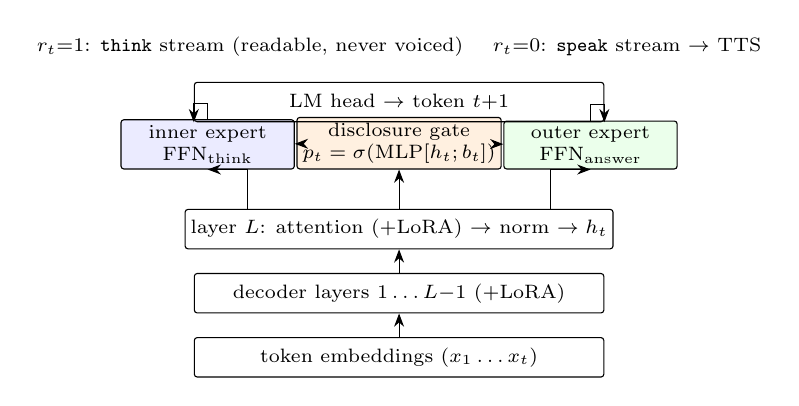
\begin{tikzpicture}[font=\scriptsize, node distance=3mm, box/.style={draw, rounded corners=1pt, minimum height=5mm, inner sep=2pt, align=center}, >=Stealth]
\node[box, minimum width=52mm] (emb) {token embeddings ($x_1\ldots x_t$)};
\node[box, minimum width=52mm, above=of emb] (layers) {decoder layers $1\ldots L{-}1$ (+LoRA)};
\node[box, minimum width=52mm, above=of layers] (attn) {layer $L$: attention (+LoRA) $\rightarrow$ norm $\rightarrow h_t$};
\node[box, fill=blue!8, above left=5mm and -14mm of attn, minimum width=22mm] (think) {inner expert\\$\mathrm{FFN}_{\text{think}}$};
\node[box, fill=green!8, above right=5mm and -14mm of attn, minimum width=22mm] (ans) {outer expert\\$\mathrm{FFN}_{\text{answer}}$};
\node[box, fill=orange!12, above=5mm of attn, minimum width=16mm] (router) {disclosure gate\\$p_t=\sigma(\mathrm{MLP}[h_t;b_t])$};
\node[box, minimum width=52mm, above=11mm of attn] (lm) {LM head $\rightarrow$ token $t{+}1$};
\node[above=2mm of lm, align=center] (out) {$r_t{=}1$: \think{} stream (readable, never voiced) \quad $r_t{=}0$: \speak{} stream $\rightarrow$ TTS};
\draw[->] (emb) -- (layers); \draw[->] (layers) -- (attn);
\draw[->] (attn.north west) ++(8mm,0) |- (think.south);
\draw[->] (attn.north east) ++(-8mm,0) |- (ans.south);
\draw[->] (attn) -- (router);
\draw[->, dashed] (router) -- (think); \draw[->, dashed] (router) -- (ans);
\draw[->] (think.north) |- ++(0,2mm) -| (lm.south west) ; \draw[->] (ans.north) |- ++(0,2mm) -| (lm.south east);
\end{tikzpicture}}
\caption{\iv{}: only the last layer's feed-forward block changes. The gate reads the last-layer hidden state $h_t$ (and optional buffer features $b_t$) and selects the expert that produces token $t{+}1$; its bit labels that token as private or public. Both streams are ordinary text.}\label{fig:arch}
\end{figure}

\subsection{Training objective}
Given a trajectory with token types $y_t\in\{\text{think},\text{speak}\}$, the loss is the token cross-entropy over both streams plus a binary cross-entropy on the gate,
$\mathcal{L}=\mathrm{CE}(\text{tokens})+\lambda\,\mathrm{BCE}(p_t, \mathbb{1}[y_{t+1}{=}\text{think}])$, with positions where the type \emph{switches} weighted $5\times$ and teacher-forced routing (the expert indicated by the label) during training. Gate accuracy at switch points is the quantity to watch: a trajectory with correct text but a gate that switches a token late voices the beginning of a private thought.

\subsection{Streaming inference and the playback simulator}
Decoding is one autoregressive loop. At each step the gate's bit decides which expert produced the logits and therefore the mode of the sampled token; \speak{} tokens are appended to the current public chunk, which is sent to TTS at newlines; \think{} tokens go to the private stream. No decode-time controller is needed. We also simulate playback with 0.03\,s per generated token and 0.35\,s per spoken word to report time-to-first-content (TTFC), the P50/P95 pause between spoken chunks, and the \emph{premature-commitment} rate (public claims later contradicted or unsupported). Decode-time overrides of the gate (``think at most $k$ tokens per block'', ``think only while audio is buffered'') are evaluated in Table~\ref{tab:budget}; they must be trained in, not imposed.

\subsection{Interleaved trajectories from existing data}\label{sec:data}
All training data are converted programmatically from public datasets; nothing is hand-annotated.
\textbf{Knights \& Knaves} \citep{xie2024kk} (6.2k puzzles, 2--8 people): the per-step search trace is the private stream; a person's verdict becomes a public chunk after the last reasoning step that mentions that person.
\textbf{MuSiQue} \citep{trivedi2022musique} (6k questions, 2--4 hops): the decomposition with retrieved passages is private; a hop's answer is disclosed after the step citing its passage.
\textbf{ConvFill} \citep{srinivas2025convfill} (67k turns): \texttt{thoughts[i]} (reasoner knowledge chunk) $\to$ private block, \texttt{response[i]} $\to$ public block, \texttt{<sil>} items (38\% of phrases) $\to$ public filler.
\textbf{DeepMath-103K} \citep{he2025deepmath}: R1 solutions split at \texttt{</think>} into private reasoning (median 1.2k words) and a reader-facing multi-paragraph solution; paragraphs are interleaved into the reasoning by numeric/LaTeX-anchor coverage (a paragraph is disclosed once all its anchors have appeared in the private stream). We also distil 1,550 problems with Qwen3-32B at high reasoning effort through a two-section prompt, plus GPT-OSS-120B and GPT-6 Astra traces for a teacher comparison.
The same conversion yields the two baselines of the protocol: \emph{Standard CoT} (all private reasoning first, then the public text) and \emph{no-think} (public text only), trained with the same recipe.

\subsection{Reinforcement learning on the disclosure policy}\label{sec:rl}
\paragraph{Infrastructure.} Rollouts come from vLLM \citep{kwon2023vllm} engines running an \iv{} model class (two-expert last layer and gate inside the forward pass); the trainer holds the policy (base + LoRA + experts + gate), recomputes the gate's decisions for each rollout with one forward pass, scores it, and after each update folds LoRA into the weights and hot-reloads the engines. On one 8-GPU node (4 engines, 4 trainer ranks) a step of 32 prompts $\times$ 8 rollouts with an 8k cap takes 3--4 minutes on A100s and about 5 minutes for 32 $\times$ 16 at 12k on H200s.

\paragraph{Objective.} GRPO-style group-normalised advantages \citep{shao2024deepseekmath} with the policy gradient applied to the sum of token log-probabilities and gate-decision log-probabilities (weight $w_\rho$), token-mean normalised, plus a KL penalty (k3 estimator) to a frozen copy of the SFT policy on both tokens ($\beta{=}0.02$) and gate decisions ($\beta_\rho{=}0.5$). Truncated rollouts are kept with a flat penalty (soft overlong punishment, $-0.5$) rather than masked.

\paragraph{Reward.} For a rollout with public text $P$ and private text $T$,
\begin{equation}
\begin{aligned}
R = {}& \mathbb{1}[\text{correct}(P)]\,\big(1 + w_Q\,Q\big) - 0.5\,\mathbb{1}[\text{truncated}] \\
 & - 0.3\,\min\!\big(1,\tfrac{n_{\text{short}}}{10}\big),
\end{aligned}
\end{equation}
where $Q\in[0,1]$ is the mean of three disclosure-quality terms: the fraction of public lines whose numeric anchors were \emph{all} derived earlier in $T$ (an entailment proxy, the same rule used to build the SFT data), $1-\min(1, n_{\text{short}}/5)$ with $n_{\text{short}}$ the number of public blocks shorter than four tokens (gate flicker), and $1-\min(1,\mathrm{FCO}/1200)$ for early first content; $w_Q{=}0.2$. Every shaping term is thus a bounded bonus available only to correct rollouts, so no disclosure pattern can be rewarded on a wrong answer. Section~\ref{sec:failures} explains how we arrived at this form.

\paragraph{Hash-reproducible sampled routing.} The SFT gate has very low entropy (on Qwen3-4B, 0.4\% of response positions have $0.02<p_t<0.98$). Under argmax routing the executed decision is deterministic while the policy-gradient term still treats it as a sample, so the update has no exploration and, with negative advantages, pushes the few uncertain logits toward and across the decision boundary, where argmax then alternates token to token (``flicker''; Section~\ref{sec:failures}). We instead sample $r_t=\mathbb{1}[p_t>u_t]$ with $u_t$ a deterministic integer hash of (token id, position), so the engine's decision is a proper sample from the gate's distribution and the trainer recomputes the identical labels without any side channel.

\section{Experiments}
\subsection{Protocol}
We follow \citet{wei2026sxs}: accuracy is judged on the \emph{public} stream only (Knights \& Knaves: every verdict correct; MuSiQue: final answer, exact match with aliases; AIME25: last \texttt{\textbackslash boxed\{\}}), decoding is greedy or Average@$k$ (mean accuracy over $k$ independent samples per problem at $T{=}1.0$, top-$p{=}1$), and waiting is measured in token indices over the generated sequence: ARI (mean index of public tokens), ABO (mean onset index of public blocks), AIRW (mean private span before each public block) and FCO (onset of the first public block with task content; filler excluded). Rows are the base model in native thinking mode and without thinking, SFT no-think, SFT Standard CoT (think-then-speak) and \iv{}, all trained on the same converted data. Test sets are 150 examples ($\pm$4 pt) for K\&K and MuSiQue and 30 problems $\times$ 4 samples ($\pm$8 pt) or $\times$ 8 ($\pm$5.6 pt) for AIME25 \citep{balunovic2025matharena}, with a 12k new-token budget (the paper uses 32k). Unfinished samples count as wrong. All rows of a table share the token budget; the base model's thinking mode is evaluated with the same 12k budget (Average@4; \placeholder{Average@8 through the same engine, running}). Models: Qwen3-1.7B and Qwen3-4B \citep{qwen3}; SFT 2,000 steps $\times$ 16 sequences (K\&K/MuSiQue), lr $2{\times}10^{-4}$ (LoRA) / $10^{-4}$ (experts, gate). Compute and software are listed in Appendix~\ref{app:infra}.

\subsection{Knights \& Knaves and MuSiQue (SFT stage)}
\begin{table*}[t]\centering\footnotesize\resizebox{\textwidth}{!}{%
\begin{tabular}{lrrrrrrrrrr}\toprule
 & \multicolumn{5}{c}{Knights \& Knaves (150)} & \multicolumn{5}{c}{MuSiQue (150)} \\\cmidrule(lr){2-6}\cmidrule(lr){7-11}
method & K\&K acc & K\&K Avg@4 & AIRW & FCO & blocks & MuSiQue acc & MuSiQue Avg@4 & AIRW & FCO & blocks \\\midrule
Qwen3-1.7B base, thinking mode & 0.413 & – & 2111 & 2114 & 0.81 & 0.408 & – & 951 & 970 & 0.94 \\
Qwen3-1.7B base, no thinking & 0.273 & – & 0 & 619 & 1.00 & 0.272 & – & 0 & 16 & 1.00 \\
Qwen3-4B base, thinking mode & 0.333 & – & 2046 & 2059 & 0.81 & 0.496 & – & 940 & 948 & 0.92 \\
SFT no-think (1.7B) & 0.580 & 0.508 & 0 & 1 & 1.00 & 0.584 & 0.600 & 0 & 1 & 1.00 \\
SFT Standard CoT (1.7B) & 0.547 & 0.533 & 177 & 270 & 1.40 & 0.592 & 0.566 & 96 & 97 & 1.00 \\
InnerVoice SFT (1.7B) & 0.520 & 0.512 & 108 & 202 & 2.73 & 0.568 & 0.542 & 39 & 40 & 2.45 \\
no e\_think input embedding (1.7B) & 0.540 & 0.527 & 106 & 189 & 2.69 & 0.592 & 0.592 & 39 & 39 & 2.41 \\
SFT no-think (4B) & 0.740 & 0.667 & 0 & 1 & 1.00 & 0.720 & 0.694 & 0 & 1 & 1.00 \\
SFT Standard CoT (4B) & 0.833 & 0.828 & 175 & 258 & 1.41 & 0.704 & 0.670 & 97 & 101 & 1.06 \\
InnerVoice SFT (4B) & 0.793 & 0.778 & 103 & 177 & 2.85 & 0.712 & 0.686 & 39 & 40 & 2.46 \\
\bottomrule\end{tabular}}
\caption{SFT-stage results on K\&K and MuSiQue (150 test examples each, $\pm$4 pt). acc = greedy accuracy on the public stream (K\&K: all verdicts correct); Avg@4 at $T{=}1$. AIRW/FCO in token indices; blocks = public blocks per example.}\label{tab:kkmq}
\end{table*}

Table~\ref{tab:kkmq} shows the mechanics: \iv{} emits 2.7--2.9 public blocks per puzzle with AIRW 103--108 tokens versus 175--177 for think-then-speak and $\sim$2,100 for the base model in thinking mode, and on MuSiQue first content arrives at token 40 versus 97 (CoT SFT) and 950--970 (base). Accuracy is preserved relative to CoT SFT, not improved, at 1.7B (greedy K\&K 0.52 vs.\ 0.55; MuSiQue 0.57 vs.\ 0.59; all within $\pm$4 pt), and at 1.7B the private stream buys nothing over a direct-answer model (no-think 0.58). At 4B thinking helps on K\&K and \iv{} sits between no-think (0.74) and CoT (0.83) at 0.79 with the private span before each public block (AIRW) cut from 175 to 103 tokens; on MuSiQue the three 4B variants tie (0.70--0.72) and \iv{} is simply the fastest. Unlike the paper, where SxS SFT loses 20--25 points before RL recovers them, our SFT-stage model stays within noise of CoT SFT, presumably because these traces are two orders of magnitude shorter and highly structured. Ablations (LoRA-only experts, a 30\% truncated-think mix) are within noise; the type embedding $e_{\text{think}}$ changes neither switching (2.69 vs.\ 2.73 blocks) nor accuracy.

\begin{table*}[t]\centering\footnotesize\resizebox{\textwidth}{!}{%
\begin{tabular}{lrrrrrrr}\toprule
decode policy & acc & think & AIRW & FCO & TTFC (s) & P50/P95 pause (s) & premature \\\midrule
nothink & 0.213 & 0 & 0 & 1 & 10.12 & 0.00 / 0.00 & 0.609 \\
budget-32 & 0.507 & 265 & 28 & 191 & 6.23 & 0.50 / 0.52 & 0.706 \\
budget-64 & 0.527 & 276 & 49 & 197 & 6.49 & 0.41 / 1.49 & 0.555 \\
budget-128 & 0.540 & 274 & 75 & 195 & 6.24 & 0.00 / 3.40 & 0.383 \\
gate & 0.520 & 283 & 108 & 202 & 6.45 & 0.00 / 5.70 & 0.272 \\
fixed-64 & 0.000 & 309 & 64 & 315 & 9.56 & 1.48 / 1.48 & 1.000 \\
stitch-64 & 0.000 & 137 & 27 & 1 & 9.12 & 0.00 / 0.00 & 1.000 \\
\bottomrule\end{tabular}}
\caption{Decode-time disclosure policies imposed on the InnerVoice 1.7B SFT model (K\&K, greedy). Caps on think tokens per block trade waiting for premature commitments; forced switches the model never saw in training (fixed-64, STITCH-like stitch-64) break it.}\label{tab:budget}
\end{table*}

Table~\ref{tab:budget} tests decode-time control. Capping private tokens per block keeps accuracy but raises the premature-commitment rate (0.71 at a 32-token cap vs.\ 0.27 for the free gate): the gate's own stopping points are the least premature. Policies that force switches the model never saw in training score zero (the forced switch lands mid-sentence and the answer expert continues the thought), and forcing the \iv{} model to skip thinking collapses it (0.21 vs.\ 0.58 for a dedicated no-think model). A buffer-aware policy therefore has to be learned, which motivates the RL stage.

\paragraph{Architecture ablation: are two experts needed?} A gate alone could label visibility on a shared feed-forward block; the two-expert design is justified only if it beats that variant. Table~\ref{tab:arch} is the comparison we consider decisive and it is \placeholder{not yet run: shared-FFN + gate at 1.7B (K\&K/MuSiQue) and 4B (DeepMath $\rightarrow$ AIME25)}.
\begin{table}[t]\centering\footnotesize\resizebox{\columnwidth}{!}{%
\begin{tabular}{lcccc}\toprule
variant & two FFN experts & gate & switching tokens & result \\\midrule
SxS \citep{wei2026sxs} & no & token-based & yes & see Sec.~\ref{sec:rlres} \\
shared FFN + BCE gate & no & yes & no & \placeholder{} \\
\iv{} & yes & yes & no & Tables~\ref{tab:kkmq},~\ref{tab:aime_sft} \\
\bottomrule\end{tabular}}
\caption{Architecture ablation isolating the contribution of the two experts from that of the gate.}\label{tab:arch}
\end{table}

\subsection{ConvFill (voice-agent turns)}
\begin{table*}[t]\centering\footnotesize\resizebox{\textwidth}{!}{%
\begin{tabular}{lrrrrrrr}\toprule
model / policy & faithful. & coher. & filler rate & blocks/turn & think & FCO & TTFC (s) \\\midrule
InnerVoice SFT, router & 4.96 & 4.18 & \textbf{0.24} & 3.05 & 41 & 69 & \textbf{4.8} \\
InnerVoice SFT, forced no-think & 4.98 & 4.08 & 0.49 & 1.00 & 0 & 74 & 13.6 \\
SFT Standard CoT (think-then-speak) & 4.96 & 4.20 & 0.33 & 1.01 & 27 & 55 & 5.1 \\
SFT no-think & 4.96 & 4.17 & 0.34 & 1.00 & 0 & 38 & 5.7 \\
\bottomrule\end{tabular}}
\caption{ConvFill (150 held-out voice-agent turns, 1.7B). Judge scores (1--5, Qwen3-4B judge) tie; behaviour differs: the router reproduces the think-a-chunk / voice-it rhythm with the lowest filler rate and earliest simulated first content (0.03 s per think token, 0.35 s per spoken word).}\label{tab:convfill}
\end{table*}

ConvFill has no gold answers, so Table~\ref{tab:convfill} reports an LLM judge (Qwen3-4B, expected value of a 1--5 score given the reference knowledge) and rule-based filler statistics on 150 held-out turns. The judge does not separate variants (faithfulness saturates at 4.96); behaviour does: the gate reproduces the dataset's think-a-chunk / voice-it rhythm (3.05 public blocks per turn), has the lowest filler rate (0.24 vs.\ 0.33--0.34) and the earliest simulated first content (4.8\,s vs.\ 5.1--5.7\,s; 13.6\,s when the same model is forced to speak without thinking, because it rambles).

\subsection{DeepMath $\rightarrow$ AIME25 (SFT stage)}
\begin{table*}[t]\centering\footnotesize\resizebox{\textwidth}{!}{%
\begin{tabular}{lrrrrrr}\toprule
method & Avg@4 & unfinished & AIRW & FCO & think tok & blocks \\\midrule
Qwen3-1.7B base, thinking (12k cap) & 0.258 & 0.66 & 10215 & 10216 & 10215 & 0.34 \\
DeepMath SFT no-think (1.7B) & 0.000 & 0.00 & 0 & 4 & 0 & 1.00 \\
DeepMath SFT Standard CoT (1.7B) & 0.075 & 0.05 & 2294 & 3221 & 3230 & 1.71 \\
DeepMath InnerVoice SFT (1.7B) & 0.175 & 0.22 & 1655 & 688 & 6950 & 4.32 \\
Qwen3-4B base, thinking (12k cap) & 0.342 & 0.62 & 10300 & 10301 & 10300 & 0.38 \\
DeepMath SFT no-think (4B) & 0.042 & 0.00 & 0 & 12 & 0 & 1.00 \\
DeepMath SFT Standard CoT (4B) & 0.183 & 0.02 & 1284 & 1536 & 1407 & 1.73 \\
DeepMath InnerVoice SFT (4B) & 0.233 & 0.17 & 1336 & 303 & 5636 & 4.74 \\
\bottomrule\end{tabular}}
\caption{DeepMath-R1 SFT evaluated on AIME25 (30 problems $\times$ 4 samples, $T{=}1$, 12k-token cap; $\pm$8 pt). Unfinished samples (no final answer within the cap) count as wrong.}\label{tab:aime_sft}
\end{table*}

On AIME25 thinking is necessary (no-think $\approx$ 0) and \iv{} beats think-then-speak at both sizes (Table~\ref{tab:aime_sft}: 0.175 vs.\ 0.075 at 1.7B, 0.233 vs.\ 0.183 at 4B) with first content at token 688 / 303 instead of 3,221 / 1,536 and 4.3--4.7 public blocks instead of 1.7. Two caveats. First, \iv{} thinks about twice as long (6.9k / 5.6k private tokens vs.\ 3.2k / 1.4k) and 17--22\% of its samples hit the cap; a budget-matched control at 1.7B gives 0.100 vs.\ 0.075 (4k cap), 0.117 vs.\ 0.042 (8k) and 0.175 vs.\ 0.075 (12k): \iv{} stays ahead at every cap, but its advantage grows with the budget because it keeps reasoning while the CoT student stops on its own at $\sim$3k tokens. Second, both are far below the base model's thinking mode (0.258 / 0.342), which however leaves 62--66\% of samples unfinished at 12k and is silent for 10k tokens---the paper's SFT-stage picture (SxS SFT 38.3 vs.\ base 66.3) at our scale.

\begin{table*}[t]\centering\footnotesize\resizebox{\textwidth}{!}{%
\begin{tabular}{llrrrrrrrr}\toprule
teacher traces (think length) & n & model & \multicolumn{3}{c}{InnerVoice SFT} & \multicolumn{3}{c}{Standard CoT SFT} \\\cmidrule(lr){4-6}\cmidrule(lr){7-9}
 & & & Avg@4 & think & FCO & Avg@4 & think & FCO \\\midrule
DeepMath R1 solutions (dataset-provided; think median 1,237 words) & 11684 & 1.7B & 0.175 & 6950 & 688 & 0.075 & 3230 & 3221 \\
DeepMath R1 solutions (dataset-provided; think median 1,237 words) & 11684 & 4B & 0.233 & 5636 & 303 & 0.183 & 1407 & 1536 \\
Qwen3-32B, default effort (think median 374 words) & 2287 & 1.7B & 0.025 & 1343 & 167 & 0.017 & 418 & 419 \\
Qwen3-32B, default effort (think median 374 words) & 2287 & 4B & 0.042 & 854 & 145 & 0.050 & 300 & 312 \\
Qwen3-32B, reasoning\_effort=high (think median 1,230 words) & 1550 & 1.7B & 0.192 & 4745 & 1298 & 0.033 & 2285 & 2208 \\
Qwen3-32B, reasoning\_effort=high (think median 1,230 words) & 1550 & 4B & 0.208 & 3570 & 614 & 0.083 & 1074 & 1047 \\
GPT-OSS-120B, reasoning\_effort=high (think median 1,132 words) (paper's teacher) & 1312 & 1.7B & 0.083 & 5673 & 831 & 0.058 & 1788 & 1730 \\
GPT-OSS-120B, reasoning\_effort=high (think median 1,132 words) (paper's teacher) & 1312 & 4B & 0.183 & 4826 & 637 & 0.075 & 1047 & 1033 \\
GPT-6 Astra, explicit <reasoning> section (median 85 words) & 542 & 4B & 0.000 & 329 & 181 & 0.000 & 304 & 302 \\
\bottomrule\end{tabular}}
\caption{Teacher-trace comparison on AIME25 (same split/alignment pipeline and SFT recipe; Avg@4, 12k cap). Long private reasoning in the teacher traces is what transfers; InnerVoice $\geq$ think-then-speak for every long-trace teacher.}\label{tab:teacher}
\end{table*}

Table~\ref{tab:teacher} varies the teacher. Private-reasoning \emph{length} is what transfers: Qwen3-32B at default effort (374 words) gives 0.025--0.042, at high effort (1,230 words) 0.192 / 0.208 from only 1,550 problems, matching 11,684 R1 trajectories; GPT-6 Astra, whose reasoning is hidden and replaced by an 85-word explicit section, gives 0.000. \iv{} is at least as good as think-then-speak for every long-trace teacher, and the CoT students consistently learn to think \emph{less} than the \iv{} students trained on identical traces (e.g.\ 2,285 vs.\ 4,745 tokens), which we read as a hypothesis rather than a finding: interleaved disclosure keeps the unfinished parts of the answer in view, so the model keeps reasoning for them.

\subsection{Reinforcement learning (Qwen3-4B)}\label{sec:rlres}
\begin{table*}[t]\centering\footnotesize\resizebox{\textwidth}{!}{%
\begin{tabular}{lrrrrrrrrrrrrrr}\toprule
reward / run & @0 & @50 & @100 & @150 & @200 & @250 & @300 & @350 & @400 & @450 & @480 & FCO & blocks & short \\\midrule
R1 (FCO bonus, SFT prompts) & 0.158 & 0.217 & 0.292 & -- & -- & -- & -- & -- & -- & -- & -- & 21 & 93.8 & -- \\
R3 (gated $Q$, KL, unseen pool) & 0.192 & 0.308 & 0.283 & -- & -- & -- & -- & -- & -- & -- & -- & 351 & 165.7 & 111.8 \\
R4 (+flicker pen., router KL 0.5) & 0.150 & 0.333 & 0.200 & -- & -- & -- & -- & -- & -- & -- & -- & 236 & 104.1 & 78.1 \\
R5 (+sampled routing), p4 32$\times$8 & 0.142 & 0.275 & 0.242 & 0.283 & 0.375 & 0.342 & 0.367 & -- & -- & -- & -- & 661 & 9.8 & 5.4 \\
R5, Greenland 32$\times$16 & 0.183 & 0.317 & 0.317 & 0.367 & 0.317 & 0.383 & 0.308 & 0.375 & 0.325 & 0.392 & 0.408 & 359 & 10.2 & 7.5 \\
\bottomrule\end{tabular}}
\caption{RL round 3 on Qwen3-4B InnerVoice: AIME25 Average@4 (n=120, $\pm$8 pt) at each evaluation step; the last three columns describe the final evaluated checkpoint (FCO, public blocks, short blocks $<$4 tokens = router flicker). R1 and R3--R4 end in degenerate disclosure (speak-everything or flicker) despite rising or flat accuracy.}\label{tab:rl}
\end{table*}

Starting from the Qwen3-32B-high \iv{} SFT model retrained without $e_{\text{think}}$ (its five step-0 evaluations spread 0.142--0.192, the $\pm$8 pt noise in action), Table~\ref{tab:rl} tracks AIME25 through five reward designs; the mechanism behind R1--R4 is in Section~\ref{sec:failures}. R5 is the only design whose disclosure profile stays intact through training. All numbers below are SFT$\rightarrow$RL on the same checkpoint, evaluated with the same 12k budget and protocol. Its small run (32 prompts $\times$ 8 rollouts, 8k cap, 300 steps on A100s) ends at 0.367 Average@4, its large run (32 $\times$ 16, 12k cap, 480 steps on H200s) at 0.408, rising from 0.183 at step 0 and staying in a 0.31--0.38 band from step 150. Table~\ref{tab:final} re-evaluates both final checkpoints at Average@8: 0.325 and 0.404. The 480-step model answers from token $\sim$470 in about ten public blocks, versus the base thinking mode's single block after 10,301 tokens, at the cost of longer private reasoning (8.3k tokens; 41\% of samples hit the 12k cap). Among samples that finish, its accuracy is 0.69 (the base model's is 0.89 on the 38\% it finishes); a 32k-budget evaluation matching the paper is \placeholder{32k-budget Average@8 for base / SFT / RL checkpoints; expected to raise all rows, run pending}.
\begin{table*}[t]\centering\footnotesize\resizebox{0.85\textwidth}{!}{%
\begin{tabular}{lrrrrrrr}\toprule
model & acc & unfin. & FCO & AIRW & think & blocks & short \\\midrule
Qwen3-4B base, thinking mode (Avg@4) & 0.342 & 0.62 & 10301 & 10300 & 10300 & 0.4 & -- \\
Standard CoT SFT (Avg@4) & 0.083 & 0.01 & 1047 & 922 & 1074 & 1.6 & -- \\
InnerVoice SFT, e\_think variant (Avg@4) & 0.208 & 0.01 & 614 & 1175 & 3570 & 3.0 & -- \\
\midrule
InnerVoice RL R5, p4 (300 steps, 32$\times$8, 8k) & 0.325 & 0.24 & 669 & 966 & 6865 & 9.4 & 5.1 \\
InnerVoice RL R5, Greenland (480 steps, 32$\times$16, 12k) & 0.404 & 0.41 & 472 & 1232 & 8333 & 10.4 & 7.5 \\
\bottomrule\end{tabular}}
\caption{Final RL checkpoints on AIME25 at \textbf{Average@8} (30 problems $\times$ 8 samples, n=240, $\pm$5.6 pt; 12k cap), with the SFT and base rows (Avg@4, n=120) for reference. Unfinished samples count as wrong.}\label{tab:final}
\end{table*}


\subsection{Comparison with \citet{wei2026sxs}}
The paper reports, for Qwen3-4B on AIME25 at a 32k budget: base 66.3 (AIRW 17,339), Standard CoT SFT 62.9, Standard CoT RL 73.8, SxS SFT 38.3 (AIRW 4,035), SxS RL 80.0 (AIRW 8,519), with GRPO on DAPO-17K at group 16, batch 32, 480+120 steps. Our numbers are not directly comparable---12k budget, 1,550 distilled SFT trajectories instead of a large multi-source corpus, LoRA plus a two-expert last layer instead of full fine-tuning, 480 RL steps on 8,918 DeepMath problems---but the shape agrees: SFT drops the model below its thinking mode, RL brings it back above, and RL roughly doubles the private reasoning per public block (our AIRW 563 $\to$ 1,232). Our SFT$\to$RL gain is +22 points against the paper's +42.

\section{What Breaks Disclosure RL, and Why}\label{sec:failures}
All runs in Table~\ref{tab:rl} share the trainer; only the reward and the prompt pool differ, which makes their failure modes informative.
\paragraph{R1: speak-everything.} Correctness plus a first-content bonus ($0.1\cdot\mathrm{FCO}/600$, paid when correct) on the 1,550 SFT problems. Group accuracy was 0.84, so in most groups the \emph{only} in-group reward variance was the FCO term; the policy learned to open a public block at token $\sim$20 and, by step 100, to carry the reasoning in the public stream (94 public blocks, FCO 21, 52\% unfinished). Accuracy rose to 0.292, but the model was no longer disclosing conclusions---it was narrating.
\paragraph{R2: dense penalties without an anchor} (run on the larger node, not in the table): penalising unsupported public lines (0.5), short blocks (0.05 each) and FCO with no KL term drove the policy first into word-level think/speak oscillation (step 50: 30 blocks, 21 short) and then into a 70-token private restatement followed by one short public paragraph (AIME 0.19 $\to$ 0.00 by step 100). Dense shaping terms are always on and consistent; correctness is sparse and noisy; GRPO optimises the former first.
\paragraph{R3/R4: flicker.} Making every shaping term a bonus gated on correctness, keeping truncated rollouts with a flat penalty, adding the KL anchor and moving to unseen problems gave clean training for 50--70 steps (R4 step 50: 0.333 with 4.4 blocks) and then word-level flicker (R4 step 100: 104 blocks, 78 short). Raising the flicker penalty and the gate KL delayed but did not prevent it. Our explanation, consistent with the training curves (gate KL and short-block counts jump together) and with the 0.4\% uncertain-position statistic, is policy-gradient instability under low-entropy routing: with argmax routing the gradient term $\nabla\log\pi(r_t)$ is non-negligible only at the few uncertain positions, and a negative advantage pushes exactly those logits toward and across zero, where argmax decoding then alternates with tiny hidden-state changes.
\paragraph{R5.} Sampled routing with a reproducible hash turns the gate update into a proper policy gradient and, with $w_\rho{=}0.2$, removes the flicker: short blocks per rollout fall from 3.8 to 0.6 over training instead of exploding, and both R5 runs keep 8--12 public blocks and FCO 400--900 on AIME25 to the end.

\paragraph{A note on gradient checkpointing.} While adding sampled routing we found that our training forward cleared the teacher-forced gate decisions before backward, so under gradient checkpointing the last layer's recomputation used the gate's own decision rather than the label on the $\sim$1\% of positions where they disagree. All 4B SFT models were trained with checkpointing and carry this small bias; the RL runs after the fix are unaffected. \placeholder{re-run of the 4B SFT without the bug and its AIME25 number}.

\section{Limitations}
Sample sizes are small (150 test examples; 30 AIME problems $\times$ 4--8 samples), single seed, and we report differences within noise as ties. Our budget (12k) is below the paper's (32k) and the base thinking mode is penalised most by it. The entailment proxy for ``unsupported disclosure'' only checks numeric and LaTeX anchors. The playback simulator uses fixed per-token and per-word costs rather than a TTS engine; \placeholder{end-to-end latency with a real streaming TTS and user study}. We did not evaluate GPQA \citep[gated;][]{wei2026sxs}, and the voice-stage rewards that use the buffer features $b_t$ (stall-aware pacing) are implemented but untrained: \placeholder{buffer-aware RL results}. Finally, \iv{} inherits every risk of the base model; the readable private stream makes its reasoning auditable but is not a safety mechanism.

\section{Conclusion}
A per-token disclosure gate over a two-expert last layer is enough to make a pretrained decoder think while it talks: it is trainable from converted existing data, runs in a standard inference engine, matches think-then-speak fine-tuning where reasoning does not matter and beats it where it does, and---once the gate is trained with a reward that cannot be gamed by wrong answers, a KL anchor and genuinely sampled decisions---RL lifts a 4B model from 0.14--0.19 to 0.40 on AIME25 at a fixed 12k budget, above its own native thinking mode, while its first public content arrives after $\sim$470 generated tokens instead of $\sim$10,000 (a pre-disclosure token count, not a measured wall-clock latency).

\bibliography{refs}

\appendix
\section{Appendix}
\subsection{Hyperparameters}\label{app:hparams}
SFT: LoRA rank 16, $\alpha{=}32$ on all attention and MLP projections; last-layer experts fully fine-tuned; gate hidden 256, output bias initialised to $-1$ (answer); loss weight $\lambda{=}1$, switch positions $\times 5$; AdamW, lr $2{\times}10^{-4}$ (LoRA) / $10^{-4}$ (experts, gate), bf16, context 4,096 (DeepMath) / 2,048 (others); K\&K+MuSiQue 2,000 steps $\times$ 16 sequences; DeepMath-R1 1,000 (1.7B) / 800 (4B) steps; Qwen3-32B-high 500 steps $\times$ 16 sequences at 4B.
RL (R5): 32 prompts $\times$ 8 (A100) or 16 (H200) rollouts per step, $T{=}1$, cap 8k / 12k, group-normalised advantages, lr $10^{-5}$ (LoRA) / $5{\times}10^{-5}$ (experts, gate), grad-norm clip 1.0, $w_\rho{=}0.2$, $\beta{=}0.02$, $\beta_\rho{=}0.5$, $w_Q{=}0.2$, FCO reference 1,200, truncation penalty 0.5, flicker penalty 0.3, prompt pool 8,918 DeepMath problems of difficulty $\geq$5 not used in SFT; AIME25 Average@4 every 50 steps through the engines.

\subsection{Compute and software}\label{app:infra}
SFT and HF-decode evaluation: single NVIDIA A100-80GB per run. RL: one 8$\times$A100-80GB node (4 vLLM 0.9.1 engines + 4 trainer ranks) and one 8$\times$H200 node; PyTorch 2.7/2.9, transformers 4.52/4.57, PEFT 0.15/0.21, vLLM 0.9.1 (custom model class and worker extension for in-place weight reload). Teacher traces via Amazon Bedrock (Qwen3-32B, GPT-OSS-120B, GPT-6 Astra). One RL step of 32 $\times$ 8 at 8k takes 3--4 min (rollout 100 s, label pass 20 s, update 90 s, weight sync 20 s).

\subsection{Phase 1: recurrent latent reasoning (null result)}\label{app:latent}
Before \iv{} we tested whether private reasoning could be replaced by $K$ recurrent passes over $M{=}8$ latent slots (an adapter with cross-attention to the context, or the LM itself as the recurrence, Coconut-style), feeding the slots as soft tokens before the answer. On three self-generated verifiable task families (arithmetic chains, templated word problems, DAG reachability) with Qwen3-1.7B/4B and matched training budgets, every $K\in\{0,1,2,4,8\}$ and five remedies (context-initialised state, mid-layer context, CODI-style self-distillation, verified intermediate-result supervision, latent-only training) landed within seed noise ($\pm$0.8 pt) of a LoRA-only direct-answer baseline (57.1\% / 69.1\%), while explicit chain-of-thought reached 80.9\% / 79.9\%. Diagnostics showed the latent state was context-independent (across-example std 0.0007; shuffling slots across examples changed nothing) and that when forced to be context-dependent the adapter could not compute the intermediates (first intermediate decoded at 23\%). This is why the private stream in \iv{} is readable text.

\subsection{Data examples}\label{app:data}
\placeholder{one K\&K, one MuSiQue, one ConvFill and one DeepMath interleaved trajectory, with gate labels}.

\makeatletter
\@ifundefined{isChecklistMainFile}{
  % We are compiling a standalone document
  \newif\ifreproStandalone
  \reproStandalonetrue
}{
  % We are being \input into the main paper
  \newif\ifreproStandalone
  \reproStandalonefalse
}
\makeatother

\ifreproStandalone
\documentclass[letterpaper]{article}
\usepackage[submission]{aaai2027}
\setlength{\pdfpagewidth}{8.5in}
\setlength{\pdfpageheight}{11in}
\frenchspacing

\begin{document}
\fi
\setlength{\leftmargini}{20pt}
\makeatletter\def\@listi{\leftmargin\leftmargini \topsep .5em \parsep .5em \itemsep .5em}
\def\@listii{\leftmargin\leftmarginii \labelwidth\leftmarginii \advance\labelwidth-\labelsep \topsep .4em \parsep .4em \itemsep .4em}
\def\@listiii{\leftmargin\leftmarginiii \labelwidth\leftmarginiii \advance\labelwidth-\labelsep \topsep .4em \parsep .4em \itemsep .4em}\makeatother

\setcounter{secnumdepth}{0}
\renewcommand\thesubsection{\arabic{subsection}}
\renewcommand\labelenumi{\thesubsection.\arabic{enumi}}

\newcounter{checksubsection}
\newcounter{checkitem}[checksubsection]

\newcommand{\checksubsection}[1]{%
  \refstepcounter{checksubsection}%
  \paragraph{\arabic{checksubsection}. #1}%
  \setcounter{checkitem}{0}%
}

\newcommand{\checkitem}{%
  \refstepcounter{checkitem}%
  \item[\arabic{checksubsection}.\arabic{checkitem}.]%
}
\newcommand{\question}[2]{\normalcolor\checkitem #1 #2 \color{blue}}
\newcommand{\ifyespoints}[1]{\makebox[0pt][l]{\hspace{-15pt}\normalcolor #1}}

\section*{Reproducibility Checklist}

\vspace{1em}
\hrule
\vspace{1em}

\textbf{Instructions for Authors:}

This document outlines key aspects for assessing reproducibility. Please provide your input by editing this \texttt{.tex} file directly.

For each question (that applies), replace the ``Type your response here'' text with your answer.

\vspace{1em}
\noindent
\textbf{Example:} If a question appears as
%
\begin{center}
\noindent
\begin{minipage}{.9\linewidth}
\ttfamily\raggedright
\string\question \{Proofs of all novel claims are included\} \{(yes/partial/no)\} \\
Type your response here
\end{minipage}
\end{center}
you would change it to:
\begin{center}
\noindent
\begin{minipage}{.9\linewidth}
\ttfamily\raggedright
\string\question \{Proofs of all novel claims are included\} \{(yes/partial/no)\} \\
yes
\end{minipage}
\end{center}
%
Please make sure to:
\begin{itemize}\setlength{\itemsep}{.1em}
\item Replace ONLY the ``Type your response here'' text and nothing else.
\item Use one of the options listed for that question (e.g., \textbf{yes}, \textbf{no}, \textbf{partial}, or \textbf{NA}).
\item \textbf{Not} modify any other part of the \texttt{\string\question} command or any other lines in this document.\\
\end{itemize}

You can \texttt{\string\input} this .tex file right before \texttt{\string\end\{document\}} of your main file or compile it as a stand-alone document. Check the instructions on your conference's website to see if you will be asked to provide this checklist with your paper or separately.

\vspace{1em}
\hrule
\vspace{1em}

% The questions start here

\checksubsection{General Paper Structure}
\begin{itemize}

\question{Includes a conceptual outline and/or pseudocode description of AI methods introduced}{(yes/partial/no/NA)}
yes

\question{Clearly delineates statements that are opinions, hypothesis, and speculation from objective facts and results}{(yes/no)}
yes

\question{Provides well-marked pedagogical references for less-familiar readers to gain background necessary to replicate the paper}{(yes/no)}
yes

\end{itemize}
\checksubsection{Theoretical Contributions}
\begin{itemize}

\question{Does this paper make theoretical contributions?}{(yes/no)}
no

	\ifyespoints{\vspace{1.2em}If yes, please address the following points:}
        \begin{itemize}
	
	\question{All assumptions and restrictions are stated clearly and formally}{(yes/partial/no)}
	NA

	\question{All novel claims are stated formally (e.g., in theorem statements)}{(yes/partial/no)}
	NA

	\question{Proofs of all novel claims are included}{(yes/partial/no)}
	NA

	\question{Proof sketches or intuitions are given for complex and/or novel results}{(yes/partial/no)}
	NA

	\question{Appropriate citations to theoretical tools used are given}{(yes/partial/no)}
	NA

	\question{All theoretical claims are demonstrated empirically to hold}{(yes/partial/no/NA)}
	NA

	\question{All experimental code used to eliminate or disprove claims is included}{(yes/no/NA)}
	NA
	
	\end{itemize}
\end{itemize}

\checksubsection{Dataset Usage}
\begin{itemize}

\question{Does this paper rely on one or more datasets?}{(yes/no)}
yes

\ifyespoints{If yes, please address the following points:}
\begin{itemize}

	\question{A motivation is given for why the experiments are conducted on the selected datasets}{(yes/partial/no/NA)}
	yes

	\question{All novel datasets introduced in this paper are included in a data appendix}{(yes/partial/no/NA)}
	partial

	\question{All novel datasets introduced in this paper will be made publicly available upon publication of the paper with a license that allows free usage for research purposes}{(yes/partial/no/NA)}
	yes

	\question{All datasets drawn from the existing literature (potentially including authors' own previously published work) are accompanied by appropriate citations}{(yes/no/NA)}
	yes

	\question{All datasets drawn from the existing literature (potentially including authors' own previously published work) are publicly available}{(yes/partial/no/NA)}
	yes

	\question{All datasets that are not publicly available are described in detail, with explanation why publicly available alternatives are not scientifically satisficing}{(yes/partial/no/NA)}
	NA

\end{itemize}
\end{itemize}

\checksubsection{Computational Experiments}
\begin{itemize}

\question{Does this paper include computational experiments?}{(yes/no)}
yes

\ifyespoints{If yes, please address the following points:}
\begin{itemize}

	\question{This paper states the number and range of values tried per (hyper-) parameter during development of the paper, along with the criterion used for selecting the final parameter setting}{(yes/partial/no/NA)}
	partial

	\question{Any code required for pre-processing data is included in the appendix}{(yes/partial/no)}
	yes

	\question{All source code required for conducting and analyzing the experiments is included in a code appendix}{(yes/partial/no)}
	yes

	\question{All source code required for conducting and analyzing the experiments will be made publicly available upon publication of the paper with a license that allows free usage for research purposes}{(yes/partial/no)}
	yes
        
	\question{All source code implementing new methods have comments detailing the implementation, with references to the paper where each step comes from}{(yes/partial/no)}
	partial

	\question{If an algorithm depends on randomness, then the method used for setting seeds is described in a way sufficient to allow replication of results}{(yes/partial/no/NA)}
	yes

	\question{This paper specifies the computing infrastructure used for running experiments (hardware and software), including GPU/CPU models; amount of memory; operating system; names and versions of relevant software libraries and frameworks}{(yes/partial/no)}
	yes

	\question{This paper formally describes evaluation metrics used and explains the motivation for choosing these metrics}{(yes/partial/no)}
	yes

	\question{This paper states the number of algorithm runs used to compute each reported result}{(yes/no)}
	yes

	\question{Analysis of experiments goes beyond single-dimensional summaries of performance (e.g., average; median) to include measures of variation, confidence, or other distributional information}{(yes/no)}
	partial

	\question{The significance of any improvement or decrease in performance is judged using appropriate statistical tests (e.g., Wilcoxon signed-rank)}{(yes/partial/no)}
	no

	\question{This paper lists all final (hyper-)parameters used for each model/algorithm in the paper’s experiments}{(yes/partial/no/NA)}
	yes


\end{itemize}
\end{itemize}
\ifreproStandalone
\end{document}
\fi
\end{document}
